\chapter{Обзор Литературы} \label{chapt1}
% ОПРЕДЕЛЕНИЕ РАДИАЦИОННОЙ НАГРУЗКИ В КОСМИЧЕСКОМ АППАРАТЕ ПРИ ПОЛЕТЕ ПО ВЫСОКОШИРОТНОЙ ОРБИТЕ

\section{Радиационная обстановка на высокоширотных околоземных орбитах. } \label{sect1_1}

Исследования радиационной обстановки в космическом пространстве связано с началом полетов автоматических аппаратов и человека в космос.  Широкое распространение технологий, связанных с использованием космической техники, а также постоянное пребывание человека в космическом пространстве во время миссий на космических станциях МИР и МКС позволило выявить ряд опасностей космических полетов, среди которых особое внимание следует уделить радиационной опасности. Значительная часть исследований физических условий в космическом пространстве проводилась в НИИЯФ МГУ \cite{logachev2007}.


Запуск 2-го и 3-го спутников Земли, с приборами, изготовленными в НИИЯФ~МГУ,  
показал принципиальную возможность полета человека в космос.  Еще из данных полученных при первых исследованиях радиационной 
обстановки был сделан вывод, что на орбите земли существуют отдельные области повышения радиационного фона (Рисунок \ldots{}). Существование данных областей связано с неоднородностями 
магнитного поля Земли и приводит к формированию области повышения потоков 
частиц в 
Южно Атлантической области \cite{logachev2007}, названной Южно-Атлантической 
Аномалией (ЮАА), как показано в статье Вернова С.Н.\cite{vernov1961}. В первом 
приближении для описания магнитного поля  Земли на высотах до 2000 км можно 
использовать представление модели смещенного диполя, этот подход позволяет 
учитывать ЮАА [Модель космоса 3 том 20стр].
%Сошлёмся на библиографию. Одна ссылка: \cite[с.~54]{Sokolov}\cite[с.~36]{Gaidaenko}. Две ссылки: \cite{Sokolov,Gaidaenko}. Много ссылок:  \cite[с.~54]{Lermontov,Management,Borozda}

Рисунок Распределение потоков частиц по данным 2-го корабля-спутника над поверхностью земного шара на высоте 320 км. (цифpы у линий дают потоки частиц в см\textsuperscript{-2} c\textsuperscript{-1}) \cite{logachev2007}.


Таким образом, магнитное поле Земли экранирует космические аппараты, находящиеся на средних широтах и невысоких орбитах порядка трехсот-четырехсот километров от поверхности Земли (именно на этих высотах поддерживается обращение космических станций). Значительный вклад, до 60\%,  в дозовую нагрузку аппараты и их экипаж получают в ЮАА [?].


Другими, важными с точки зрения радиационной обстановки, являются приполярные области [Горчаков Е.В. \textbf{Внешний радиационный пояс и полярные сияния. }\emph{Искусственные спутники Земли, 1961, вып. 9, с. 66-70.}].

При выборе более высокоширотных и высоких орбит дополнительного внимания требуют области полярных шапок, так как в этих областях границы радиационных поясов Земли ближе к поверхности. Даже на небольших высотах, начиная от 300 км в интервале геомагнитных широт 55-70 наблюдается резкое возрастание интенсивности излечения и частицами, составляющими этот внешний радиационный пояс являются электроны различных энергий, их поток достигает 10\textsuperscript{5} см\textsuperscript{-2} сек\textsuperscript{-1} стер\textsuperscript{-1} [Исследования космических лучей и земного корпускулярного излучения при полетах ракет и спутников; УФН, т. 70, вып. 4, 585 (1960)]. При солнечных событиях в этих областях создаются условия для многократного повышения потоков частиц, что может привести к необходимости специальных мер по предотвращению чрезмерной радиационной нагрузке на экипаж космического аппарата.

\subsection{Вопросы, требующие детального исследования}
Происхождение и динамика потоков релятивистских электронов до сих пор вызывает активный интерес мирового сообщества, несмотря на множество исследований  за более чем пол века исследований \cite{Gussenhoven1997,Borovsky2010,Holeman1991,Miyoshi2011,Chen2016,Turner2013,Brautigam2001,Borovsky2010a,Gussenhoven1995,Borovsky2011,Baker2013,Mullen1998,Chen2014,Morley2010,Potapov2014,Denton2010}. Этот интерес определяется в первую очередь радиационной опасностью, которую представляют экстремально высокие потоки электронов для аппаратов на орбитах полярных спутников.

Некоторые исследования показывают связь энергичных электронов на геостационарной орбите со скоростью солнечного ветра и с УНЧ излучением\cite{potapov2012}. Также есть подтверждения, что на L \~ 2,75 могут существовать долгоживщие дополнительные узкие радиационные пояса, населенные электронами с енергиями более 6 МэВ \cite{lazutin2012}. 
Другие исследователи связывают наличие на внутренних ультра-релятивистских электронов с мощьными электромагнитными ионно-циклотронными волнами (EMIC) \cite{Shprits2013} 
%\newpage
%===============================================================================

\section{Методы регистрации дозы ионизирующих излучений} \label{sect1_2}

Среди методов регистрации ионизирующих излучений можно выделить несколько наиболее используемых, это газовые ионизационные детекторы, в том числе пропорциональные и газоразрядные счетчики, сцинтилляционные детекторы, полупроводниковые детекторы, трековые детекторы. Приборы спектрометры заряженных частиц, спектрометры нейтронов.

Первые эксперименты в космосе по измерению радиационных условий предполагали использование ионизационных камер достаточно большого размера (десятки см\textsuperscript{3}) к этим приборам относятся Р-16 и ионизационные камеры работавшие на шаттлах\cite{Dorman2004}. Современные детекторы радиации в основном строятся на основе полупроводниковых детекторов, хотя ионизационные камеры являются удобным референсным методом, который позволяет провести непрерывный временной ряд исследований вплоть до исследований на первых ИСЗ.

%\newpage
%===============================================================================

\section{Приборы для радиационного мониторинга в космосе} \label{sect1_3}

Дозиметрические и радиационные исследования в космосе не теряют актуальности на протяжении полувека космической эры человечества, это подтверждают актуальные  конференции WRMISS, COSPAR. Большая часть дозиметрических измерений в космосе происходит на космических станциях и в частности на МКС. 
В первую очередь детекторы радиации разделяются на пассивные и активные, хотя такое разделени условно так как некоторые термо-люминисцентные детекторы и баббл-детекторы можно отнести к активным - они позволяют проводить быстрое считывание данных о дозах на борту космического аппарата. 
%\newpage
%===============================================================================

\subsection{Пассивные детекторы} \label{subsect1_3_1}

Получение информации с пассивных детекторов происходит после накопления порции измерений и требует прерывания цикла измерения. По принципу регистрации излучения они подразделяются на трековые детекторы, термолюминисцентные и эмульсионные.


CR-39 тканеэквивалентный трековый детектор \cite{Zhou2008}.


TLD-100, -600, -700, OSLD Люминисцентные детекторы \cite{Zhou2010}.


BR\&Bya type NPE FILM фотографическая эмульсия


Pille портативная считывающая система[(Apathy et al., 2002, Apathy et al., 2007]


EVARM детектор MOSFET 


Матрешка-Р ионизационная камера [Machrafi, R., Garrow, K., Ing, H., et al. Neutron dose study with bubble detectors aboard the International Space Station as part of the MATROSHKA-R experiment. Radiation Protection Dosimetry 133 (4), 200--207, 2009]



%\newpage
%===============================================================================
\subsection{Активные детекторы} \label{subsect1_3_2}

Для радиационного мониторинга в космическом пространстве используются счетчики частиц, спектрометры и дозиметры. Следует отметить что первые схемы такого рода устройств были предложены еще на заре космических исследований[Маркелов В.В., Редько В.И. Высокочувствительный дозиметр космических излучений. Космические исследования, 1982, т. 19, номер 2, с. 316-319.] и на данный момент являются незаменимым средством любой космической миссии с участием человека.

К числу полупроводниковых дозиметров относятся приборы ДБ-8, DOSTEL, LIULIN, REM/MPT. Все эти приборы используют принцип регистрации поглощенной дозы в полупроводнике – кремнии, толщиной 300 мкм.  

\subsubsection{ДБ-8}

Дозиметр Бортовой (ДБ) является развитием ряда дозиметрических инструментов применявшихся на различных космических аппаратах для исследовательских целей и штатной работы. ДБ предназначен для регистрации временных вариаций мощности поглощенной дозы и плотности потока частиц СКЛ, ГКЛ, РПЗ. ДБ является детектирующими блоками Системы контроля радиационной (СРК) обстановки ПТК и МКС.

В СРК для МКС используется четыре блока ДБ, что позволяет получить информацию о неоднородности радиационного поля в различных отсеках МКС. 

Регистрируемые данные:
\begin{itemize}
	\item 
	Поглощенная доза в диапазоне - от~10\textsuperscript{-5}~Гр  до~10\textsuperscript{+1}~Гр;  
	\item  
	Мощность поглощенной дозы в диапазоне - от $10^{-10}$~Гр/с  до~$5\cdot10^{-5}$~Гр/с;
	\item  
	Плотность потока частиц в диапазоне от~1 до~$ 10^3 $~частиц/(см$^2\cdot$ с);    		
\end{itemize}

Внешний вид ДБ представлен на рисунке \ref{fig:db}.

\begin{figure}
\centering
\includegraphics[width=0.7\linewidth]{images/db}
\caption{}
\label{fig:db}
\end{figure}

Прибор содержит 2 узла детектирования, вычислительный блок, блок управления и блок вторичного питания. Оба полупроводниковых детектора в узлах детектирования расположены  параллельно,  образуя телескоп, такая схема построения прибора была использована для получения информации о ЛПЭ частиц, прошедших одновременно через оба детектора.         


Обмен информацией c ДБ обеспечивается по интерфейсу RS-422. Объем целевой информации 2 Мбайта в сутки. Питание ДБ осуществляется постоянным током c напряжением $ 27^{+7}_{-4} $ В. 

\begin{itemize}
\item Энергопотребление ДБ не более 2 Вт.
\item Масса блока 0,25 кг.
\item Габариты ДБ 85×40×100 мм. 
\item Ресурс ДБ  60000 ч, срок службы 12 лет.
\end{itemize}


Поглощенная доза регистрируется узлами с полупроводниковыми детекторами. Для получения информации о величине поглощенной дозы используется принцип регистрации величины заряда в объеме полупроводника, пропорционального энерговыделению в данном объеме. Методы преобразования сигналов с детекторов в цифровую форму и последующая обработка их на микроконтроллере остаются аналогичными алгоритмам, использованным в приборах ДБ-8, ДБ-8М, ДЭПРОН.  


\subsubsection{Liulin}

Детекторы серии Liulin используются с 1988 года, когда их первое поколение было использовано на борту космической станции МИР \cite{Caffrey2011}. Liulin-4 не последний прибор в этой серии, но его простое устройство и компактные размеры обеспечивают удобство использования для многих конкретных задач. Этот спектрометр состоит из единственного кремниевого детектора, зарадочувствительного предусилителя, микроконтроллера и флэш-памяти. Насыщенный литием кремниевый детектор имеет толщину 0,3 мм и площадь 2 см\textsuperscript{2}. В приборе установлен 12-ти битный АЦП, но только 8 бит из них используется для получения 256 канального спектра энерговыделения за выбранный интервал времени накопления: от 10 до 3539 с. Амплитуда импульса определяется после предусилителя и разделяется по 256 энергетическим каналам, начинающимся с 0,02 МэВ до 20 МэВ. Выделение энергии, большее 20 МэВ записывается в наибольший энергетический канал \cite{Dachev2002} .


Для определения дозы в данном типе детектора энерговыделение в каждом канале определяется умножением счета в детекторе на энергию канала. Эти результаты делятся на массу объема детектора и суммируются для определения общей дозы по всем каналам \cite{Dachev2002}. Записанная форма спектра энерговыделения может предоставить дополнительную информацию относительно природы доминирующего радиационного поля (ЮАА, ГКЛ и др. ), но не является достаточно подробной для определения ЛПЭ воздействующей радиации \cite{Caffrey2011}. 


Размер и портативность спектрометра типа Liulin-4 делает его жизнеспособным кандидатом для активной персональной дозиметрии во время солнечного события, но ограничения в возможности определения эффективной ЛПЭ и эквивалентной дозы предотвращают вытеснение методов пассивной дозиметрии. Liulin-4 существует во многих модификациях и с многими опциями и может работать как на химическом источнике тока, так и на непрерывном питании, функционировать как с внешним ЖК-дисплеем так и без него, и может включать GPS-приемник \cite{Dachev2002}.	

Впоследствии был разработан также Liulin-5 основным отличие которого является телескоп из трех полупроводниковых детекторов.

\subsubsection{DOSTEL}

DOSTEL -- Дозиметрический полупроводниковый телескоп был разработан в 1995 году как малый телескоп частиц для использования на миссиях космических шаттлов к космической станции МИР. Прибор включает в себя два кремниевых детектора по технологии PIPS, расположенных как телескоп [Beaujean, R., и др. 2002]. Каждый детектор имеет толщину 0,315 мм с чувствительной зоной 6,93 см2, зазор в 15 мм между детекторами дает геометрический фактор 824 см\textsuperscript{2}ср (единица измерения определяется чувствительной площадью детектора и полем зрения) для детектирования совпадающих событий [Beaujean, R., и др. 2002]. Каждый детектор соединен с зарядочувствительным усилителем через интегрирующую емкость, двух стадийным усилителем импульсов, двумя пиковыми детекторами, двумя RC-фильтрами для снижения уровня шумов и 8-ми битным АЦП. Такая компоновка позволяет поводить анализ амплитуд импульсов отдельно для высокого и низкого энергетического диапазона [Beaujean, R., и др. 2002].


Когда совпадающее событие записано обоими детекторами, становится возможным определить ЛПЭ падающего излучения. Так как известно, что траектория частицы ограничена конусом возможных направлений, средняя толщина детектора может быть использована для оценки длины трека частицы. Делением энерговыделения на среднюю длину свободного пробега, для данного детектора 0,364 мм [Beaujean, R., и др. 2002] с плотностью 2,33 г/см\textsuperscript{3} [Knoll GF, Radiation detection and measurement, third edition, Wiley: 2000, p802  на странице 357]  можно получить приближенное значение ЛПЭ. Результат таких вычислений нормируется на известный коэффициент для перехода от ЛПЭ кремнии к ЛПЭ в воде, таким образом прибор DOSTEL записывает ЛПЭ в диапазоне от 0,1 до 240 кэВ/мкм [Beaujean, R., Kopp, J., Burmeister, S., et al. Dosimetry inside MIR station using a silicon detector telescope (DOSTEL). Radiation Measurements 35, 433--438, 2002].


\subsubsection{REM/MPT}

Существенным отличием установленного NASA на МКС прибора Radiation Environment Monitor (REM) от других полупроводниковых дозиметров  является позиционно-чувствительная система считывания энерговыделений в детекторе. Эта особенность при телескопическом расположении детекторов позволяет производить значительно более точные оценки энерговыделения каждой частицы с помощью дополнительной информации о угле падения частиц. Каждый детектор представляет собой матрицу 256 X 256 пикселей размером 14х14 мм, и считывается со скоростью до 850 кадров/с.

Прибор REM включает сенсорные платы Medipix 3-го поколения. Medipix 1, 2 и 3го поколения это серия пикселизованных детекторов фотонов и заряженных частиц разрабатываемых с 1990-х годов большой коллаборацией институтов под эгидой CERN. На основе данных микросхем были построены приборы регистрации радиации для МКС с 2013 года и для первых тестов многоцелевого аппарата Орион в 2014 году.

Обработка сигнала с каждого пикселя производится поэлементно и реализована на Asic микросхеме ридаут Timepix. На данный момент известно, что исследования на борту МКС продолжатся в марте 2017 году, а разработкой новой аппаратуры занимается Европейская компания Advacam, производящая микросхемы Medipix. Для этой цели разрабатывается прибор Miniaturized Particle Telescope (MPT)\cite{Fry2016} - представляет собой телескоп из двух детекторов построенный на основе Timepix технологии \cite{Kroupa2015}, и по сути представляет собой два прибора REM. 

Для миссии на МКС прибор оснащен двумя USB коннекторами и подключается к ноутбуку, данные считываются ежедневно а обработка данных будет производится на Земле. В перспективе данный прибор рассматривается как основное дозиметрическое средство на борту КА Орион, полеты которого запланированы с сентября 2018 года.


\subsubsection{ELFIN}
Прибор ELFIN входит в состав аппаратуры КА Ломоносов и является спектрометром заряженных частиц в отличии от других описанных приборов. Прибор состоит из двух полупроводниковых телескопов с алюминиевой и танталовой защитой, которая по мнению разработчиков прибора будет необходима и достаточна для работы в радиационных поясах\cite{VassilisAngelopoulos}.

\begin{figure}
	\centering
	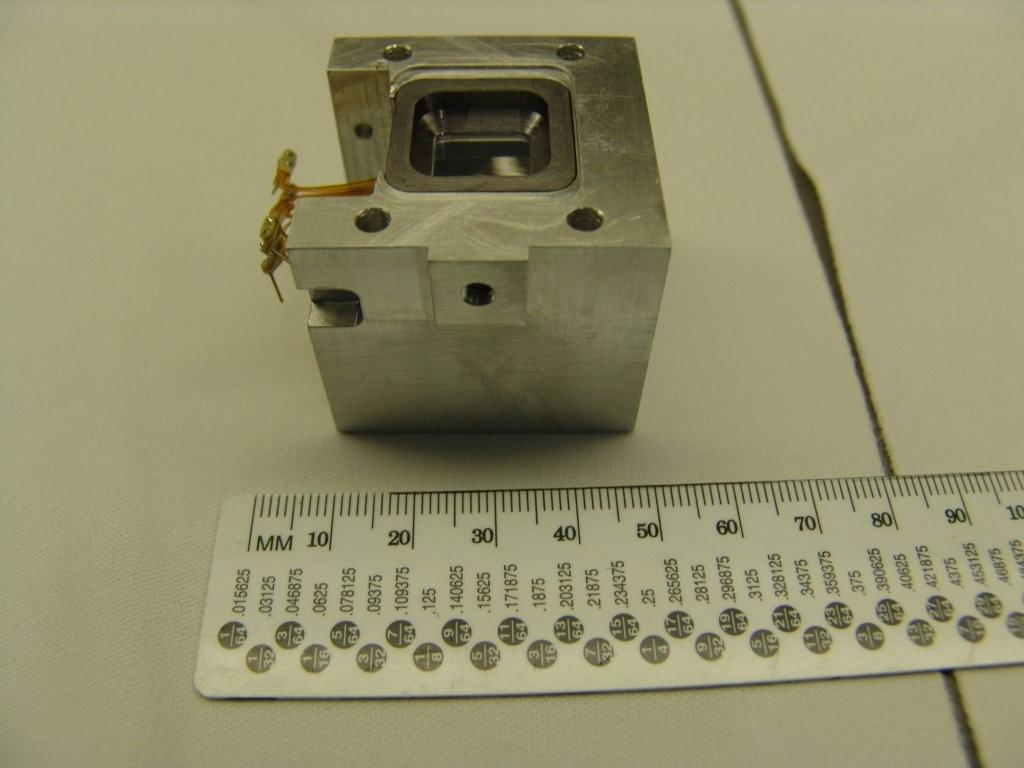
\includegraphics[width=0.49\linewidth]{images/elfin/DSC04260}
	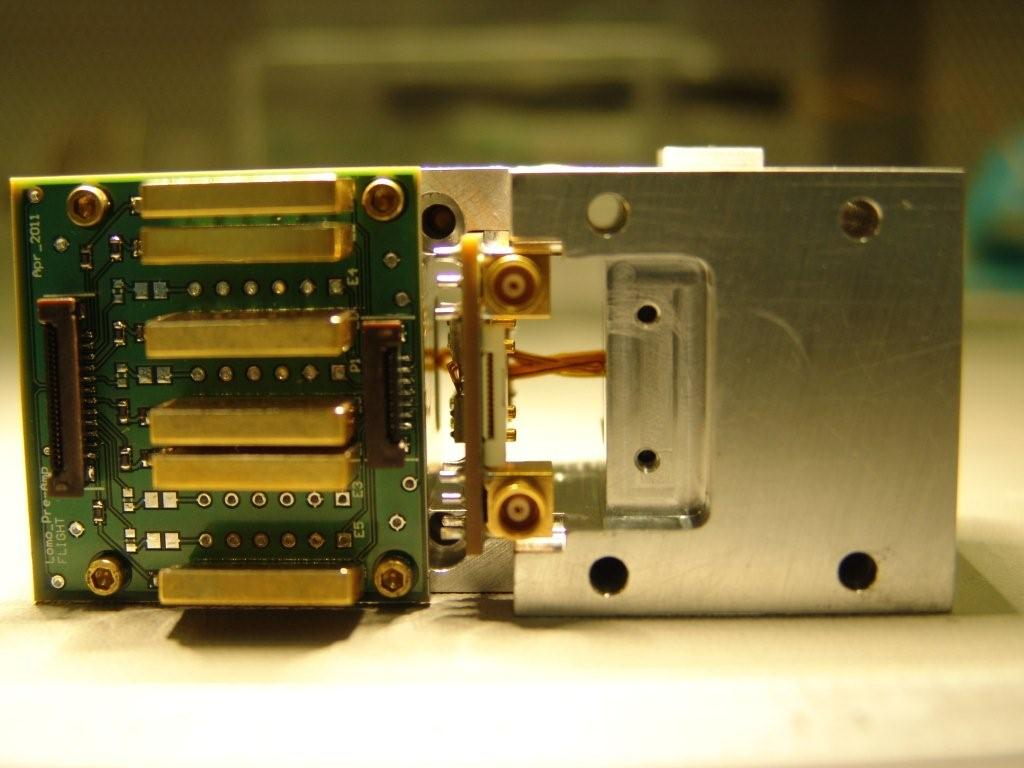
\includegraphics[width=0.49\linewidth]{images/elfin/DSC04287}
	\caption{Устройство телескопа детекторов для электронов с входным окном (слева). 	Плата предусилителей со сборкой плат электроники (справа). }
	\label{fig:dsc04260}
\end{figure}


Параметры прибора :
\begin{itemize}
	\item Диапазон измерения электронов: 50 кэВ до 4 МэВ
	
	\item Диапазон измерения ионов: 50 кэВ до 500 кэВ
	
	\item Геометрические факторы:
	
	\begin{itemize}
		\item Электроны: 0.04см$ ^{2}\cdot $ср
		
		\item Ионы: 0.003см$ ^{2}\cdot $ср
	\end{itemize}
	
	
	\item dE/E < 50\%
	
	\item Масса прибора менее 1.5 кг включая защиту детектора 1.2 см из Al+Ta
	
	\item Габариты 85 x 80 x 80 mm
\end{itemize}

В состав прибора входит магнитометр, необходимый для выяснения связи локальных магнитных условий в месте нахождения спутника и потоков электронов, покидающих радиационные пояса. С целью выявления популяции высыпающихся частиц ось телескопов прибора направлена примерно в конус потерь - на 60 линейных градусов от зенита.




\subsubsection{MSL/RAD}
Прибор Radition Assesment Detector (RAD) предназначен для оценки радиационных условий на Марсианской лаборатории Curiosity. Он состоит из детектора заряженный и нейтральных частиц\cite{Zeitlin2016}. Этот первый прибор для измерения спектра частиц и мощности дозы на пути к марсу и на его поверхности \cite{Matthia}.

RRMD-III Determines path length with PSDs [Doke et al. (2001, 2004)]


Liulin-5 Assumes mean-chord-length across FOV in LET calculation [Semkova et al. (2004, 2007)]


Liulin Phobos Assumes mean-chord-length; orthogonal telescopes [Dachev et al. (2009)]


CPDS Determines path length with PSDs; can determine species for C, N, and O particles [Lee et al. (2007)]


TEPC Assumes mean-chord-length for all angles; LET assumed equal to y (Lineal energy) [Badhwar et al. (1996), Gersey et al.(2002, 2007)]


R-16 Pulse-type ion chamber: 1 pulse per 5 mrad; shallow and deep dose rates; assumes average LET [Mitricas et al. (2002), Badhwar (2000)]


BBND Heavy system; short-term experiment; requires 3He Koshiishi et al. (2007), Matsumoto et al. (2001)

\subsubsection{SEISS}
Группа радиационных приборов SEISS установлена на GOES-R (GOES-16)\cite{Goodman2013}, который запущен 19 ноября 2016 года. 
Пакет приборов Seiss состоит из: детектора тяжелых ионов  (EHIS), детектора частиц РПЗ - высокого и низкого (MPS-HI и MPS-LO) и детектора солнечных и галактических протонов (SGPS). Планируется что данные из Seiss будут использоваться для предупреждений о опасных явлениях космической погоды, а также улучшит прогнозы потоков энергичных частиц. 

\subsubsection{MEPED}
Сеть полярных операционных спутников Земли (POES) полярно-орбитальных космических аппаратов представляет собой комплекс спутников с наиболее близкими орбитами к орбите Ломоносова и поэтому схожими по радиационным условиям полета. Особый интерес для магнитосферных исследований представляет подсистема Space Environmental Monitor, предназначенная для измерения потоков частиц на низкой околоземной орбите, сейчас она представлена ​​в обновленной конфигурации (SEM -2), эта подсистема является содержит приборы среднего протонного и электронного детекторов (MEPED).
В состав MEPED входят в общей сложности восемь приборов в диапазоне от 30 кэВ до 200+ МэВ (для протонов) и от 30 до 2500 кэВ (для электронов).

Интересно, что низковысотные, полярно-орбитальные спутники NOAA POES проявляют побочный отклик на релятивистские электроны в приборе MEPED\cite{Yando2011}.
\begin{figure}
	\centering
	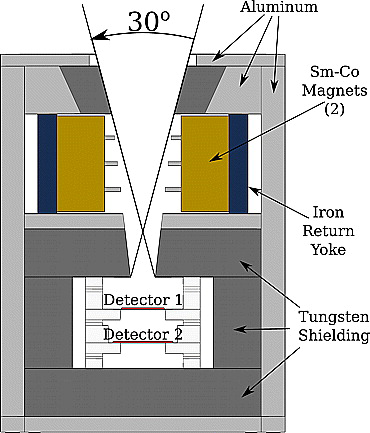
\includegraphics[width=0.3\linewidth]{images/jgra21383-fig-0002}
	\caption{Схема прибора протонного телескопа MEPED, показанного в поперечном разрезе.\cite{Yando2011}}
	\label{fig:jgra21383-fig-0002}
\end{figure}


\subsection{Детекторы нейтронов} \label{subsect1_3_1}


Достоверно известно что нейтроны также вносят ощутимый вклад в эквивалентную дозу и по разным оценкам достигает 20-30\% \cite{Dudkin1990}, а для эффектов обусловленных ядерным взаимодействием (в том числе повреждения ДНК, эффектов пробоя в микроэлектронике и биологической эквивалентой дозе) может достигать 50-60\% \cite{Armstrong2001}. Полупроводниковые детекторы имеют низкую чувствительность к нейтронному излучению и их не достаточно для регистрации ожидаемых потоков нейтронов. В НИИЯФ МГУ также разрабатывались приборы для контроля уровня нейтронного излучения  /[27],\cite{Shavrin2002}

Особенно интересны радиобиологические исследования проведенные ИМБП \cite{Shurshakov2016} на МКС с использование тканеэквивалентного фантома Матрешка, показывающие что вклад нейтронов в дозу может достигать 28\%.  Исследования при этом производились по методике определения количества пузырьков в ``Баббл-дозиметре''.

[26]  Севастьянов В.Д., Тарновский Г.Б., Лягушин В.И.  Измерение энергетического спектра нейтронов на орбитальной станции “МИР”.  Космические исследования, т.35, №2, 1997, с. 216-220.

[27]  М.И. Панасюк, П.И. Шаврин, О.Ю. Нечаев, Л.С. Братолюбова-Целукидзе, Т.Р. Маркелова, М.А. Сергеева. Многоцелевой детекторный модуль для регистрации нейтронов в околоземном пространстве. Препринт 90-13/159 НИИЯФ МГУ, 1990 г.

Также известно что счетчики нейтронов используются на орбите Марса и позволили получить важный научный результат о наличии воды на поверхности Марса.  Этот  результат получен с помошью прибора FREND \cite{Sanin2012}.

%\newpage
%===============================================================================
\section{Математическое моделирование дозиметрических приборов для космических условий}

Математическое моделирование широко применяется на всех этапах создания исследовательских проборов предназначенных для использования в условиях космоса. В первую очередь оно необходимо на этапе проектирования аппаратуры для выбора характеристик регистрирующих радиацию модулей исходя из поставленных экспериментальных задач [ Luszik-Bhadra M.  et . al . ,  2009,  Hassler  D et .  al . ,  2008 ]. На последующих шагах разработки аппаратуры математические методы используются при верификации результатов калибровочных и градуировочных испытаний на источниках ИИ и ускорителях заряженных частиц [Zeitlin C et . al ,  2010]. Также одним из основных применений является уточнение функции отклика прибора во время штатной работы [C. Zeitlin et al . 2010]. 

Существуют также доводы, показывающие необходимость сравнения результатов моделирования с \cite{Matthia}.


Среди математических методов моделирования взаимодействия ИИ и нейтральных излечений с материалами и детектирующими модулями приборов следует отметить наиболее используемые программные пакеты, основанные на методе Монте-Карло:


\begin{description}
	\item[GEANT4] комплекс программ для моделирования прохождения частиц через вещество\cite{Allison2006}
	\item[SHIELDOSE ] система расчетов доз за секционированной защитой \cite{SeltzerS.M.1980}
	\item[PHITS] Система расчета перемещений частиц и тяжелых ионов, 
	разработана в Японии и Австрии%particle and heavy ion transport code system
	\item[FLUKA] система широко использующаяся в CERN для широко круга задач и 
	первую очередь для медицинских приложений\cite{Fasso2003, fluka2014}.
\end{description}

Далее рассмотрен только пакет Geant4, так как в настоящей работе именно этот пакет 
был выбран для расчетов. 


\subsection{GEANT4}

Данная система математического моделирования разрабатывается для нужд работы 
ЦЕРН и активно используется в ряде областей науки, медицины и технологии 
\cite{Agostinelli2003}.
К настоящему моменту система Geant4 развилась настолько, что от основной ветки 
разработки отделилось несколько специализированных продуктов, использующих 
только ядро системы для расчетов распространения частиц. Основные направления 
развития это микродозиметрические исследования(GEMAT), применение к 
распространению и 
воздействия космического излучения(GRAS, PLANETOCOSMICS), оптимизация 
экранирования (MULASSIS \cite{Lei2002} и SSAT). 

Следует отметить что многие из упомянутых программ организованы в единый комплекс Spenvis,
 и особенно применим для нашего случая  Geant4 Radiation Analysis for Space (GRAS).

%\newpage
%===============================================================================
\section{Возможности КА Ломоносов в продолжении ряда российских исследований радиационной обстановки}

На многих российских пилотируемых кораблях со времен первого полета человека в космос устанавливались дозиметрические приборы, изготовленные в НИИЯФ МГУ, исчерпывающий список и результаты этих экспериментов можно найти в монографии Ю.И. Логачева 2007г \cite{logachev2007}. Отличительной чертой данного эксперимента является возможность прозондировать более высокие широты по сравнению с орбитами таких комплексов как станция МИР и МКС. 

Вторым но не менее важным моментом является уникальное сочетание многих исследовательских приборов в одном аппарате, такое сосредоточение позволит получить уникальную информацию о всех параметров исследуемых явлений, будь то гамма вспышки земного или неземного происхождения, или транзиентные явления в верхней атмосфере - такие как эльфы и спрайты. Дозиметрический прибор поможет отфильтровать сбойный явления связанные с повышением уровня радиации и отделить их от ценных данных. И наоборот, дать новую информацию о явлениях в авроральных областях, высыпаниях во внешнем радиационном поясе.
На борту спутника кроме прибора ДЭПРОН установлены два прибора позволяющие регистрировать различные компоненты радиационной нагрузки, это БДРГ --- Блок детектирования рентгеновского и гамма излучения (НИИЯФ МГУ), ELFIN (UCLA и IGPP) --- прибор для обнаружения высыпаний электронов и исследования магнитных полей содержащий детектор электронов и ионов (EPD-E и EPD-I), наряду с магнитометром. Такая тройка приборов позволяет при небольшом весе проводить измерения множества  параметров радиационной обстановки.



\begin{figure}

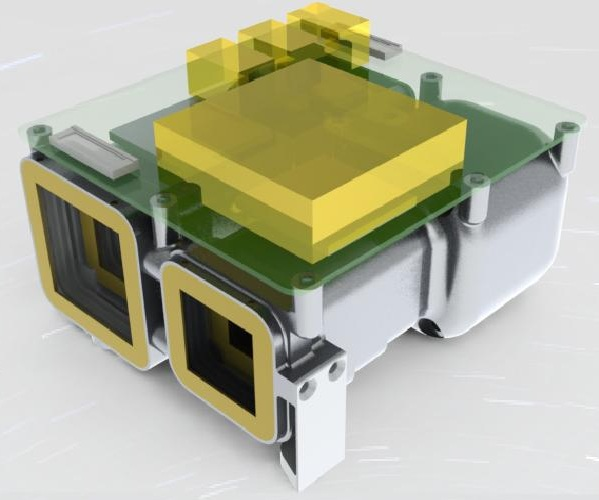
\includegraphics[width=0.7\linewidth]{images/EPD_Brochure}
\caption{}
\label{fig:epdbrochure}
\end{figure}

%\centering
%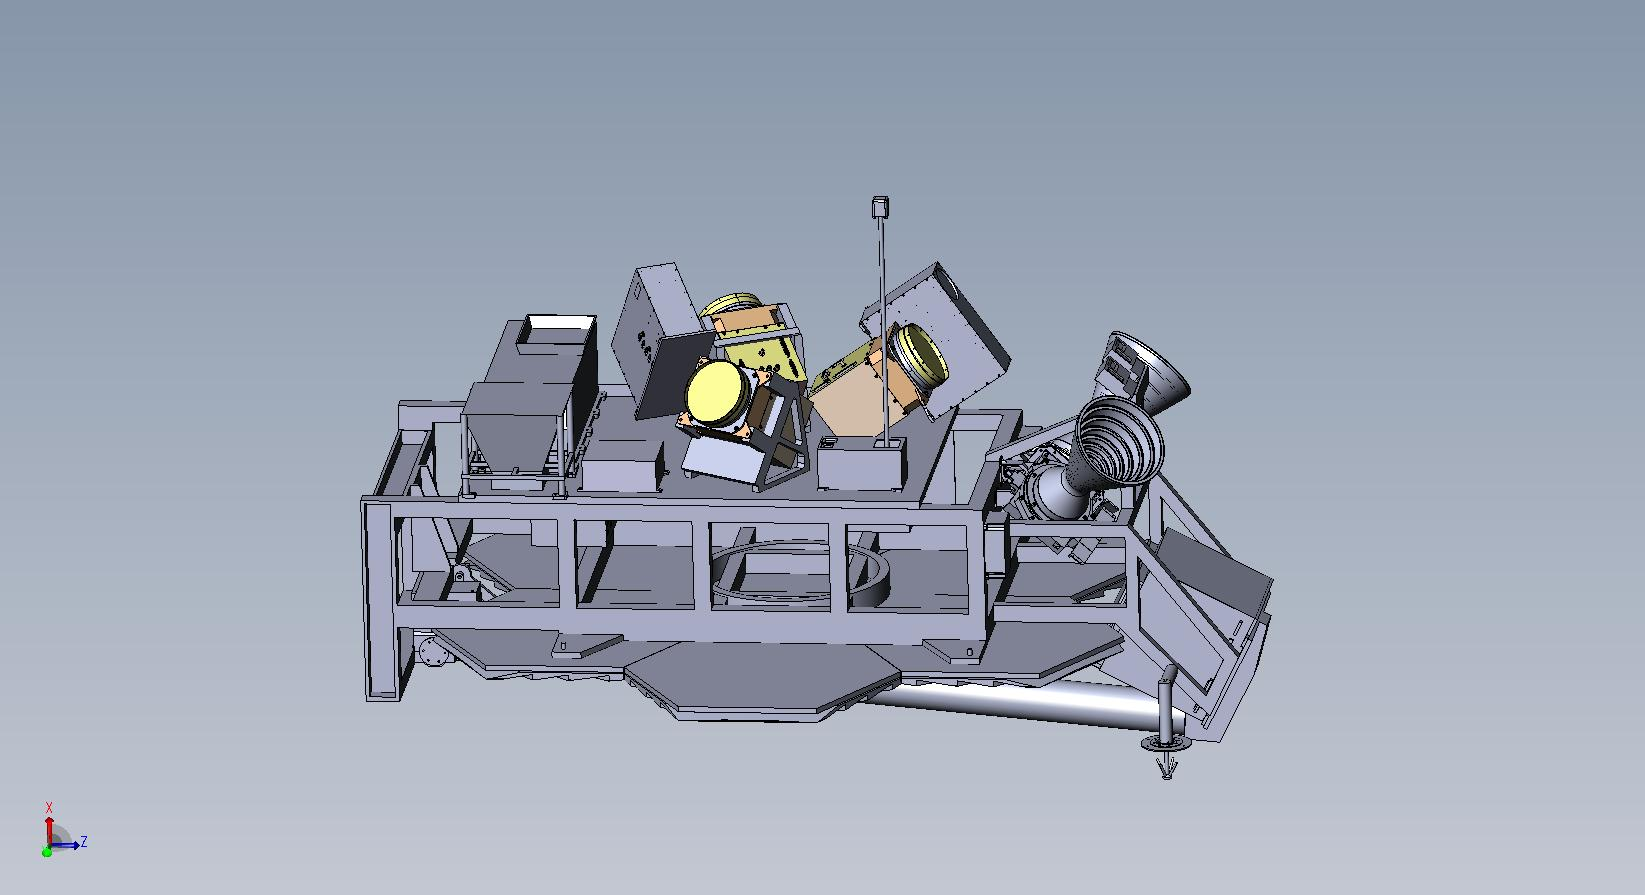
\includegraphics[width=0.8\linewidth]{images/lomonosov2}
%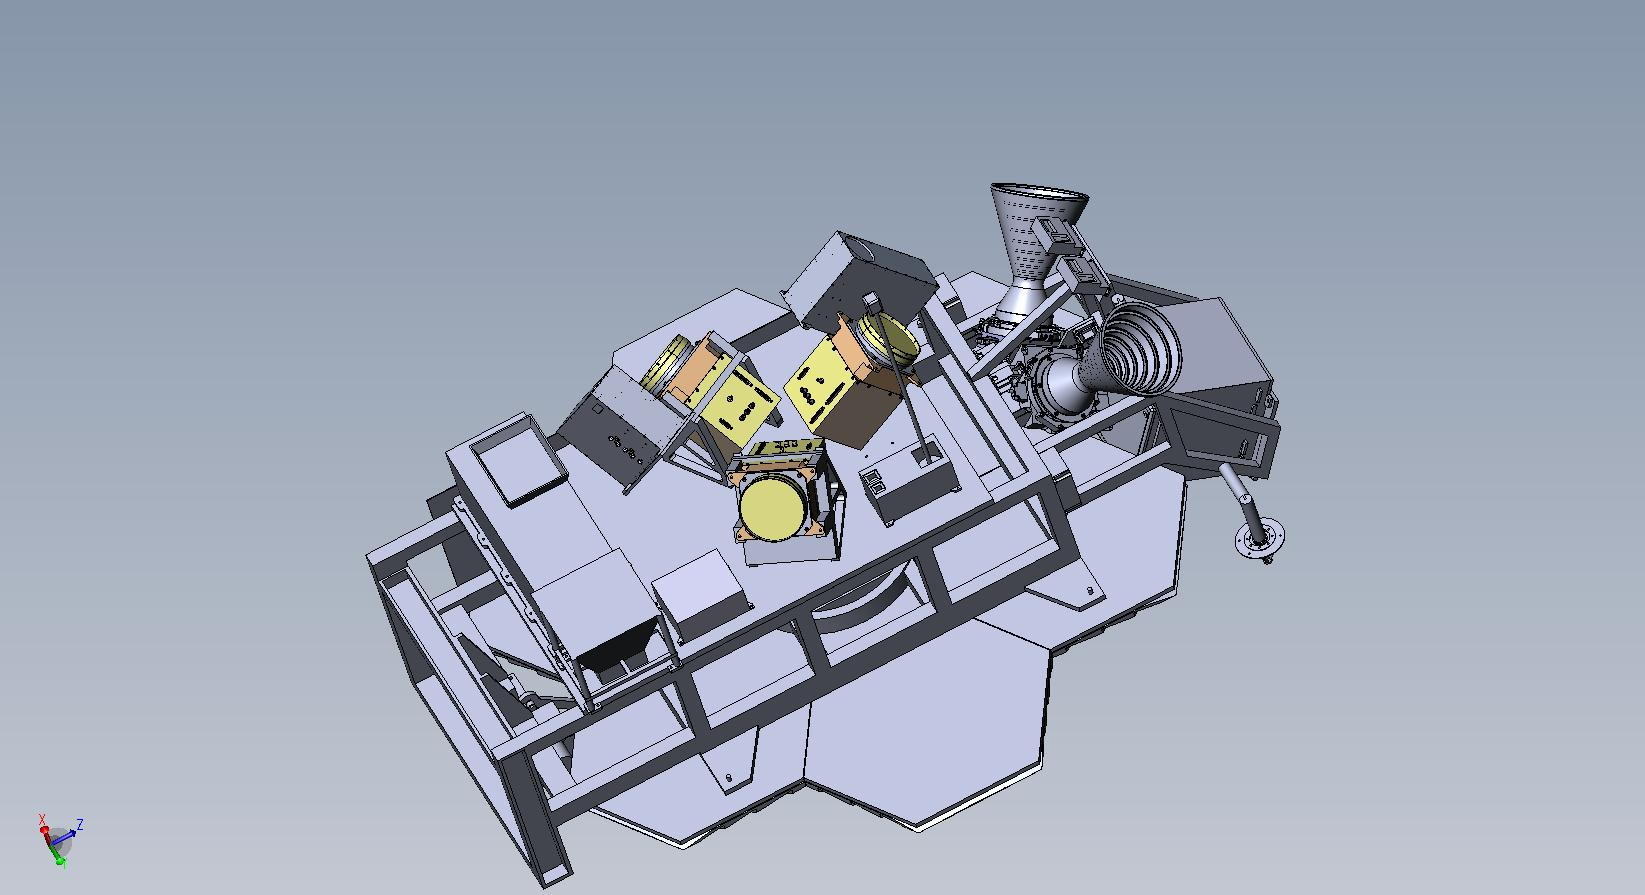
\includegraphics[width=0.8\linewidth]{images/lomonosov1}
%\caption{Внешний вид спутника Ломоносов старый}
%\label{fig:lomonosov2}
%\end{figure}

\begin{figure}
\centering
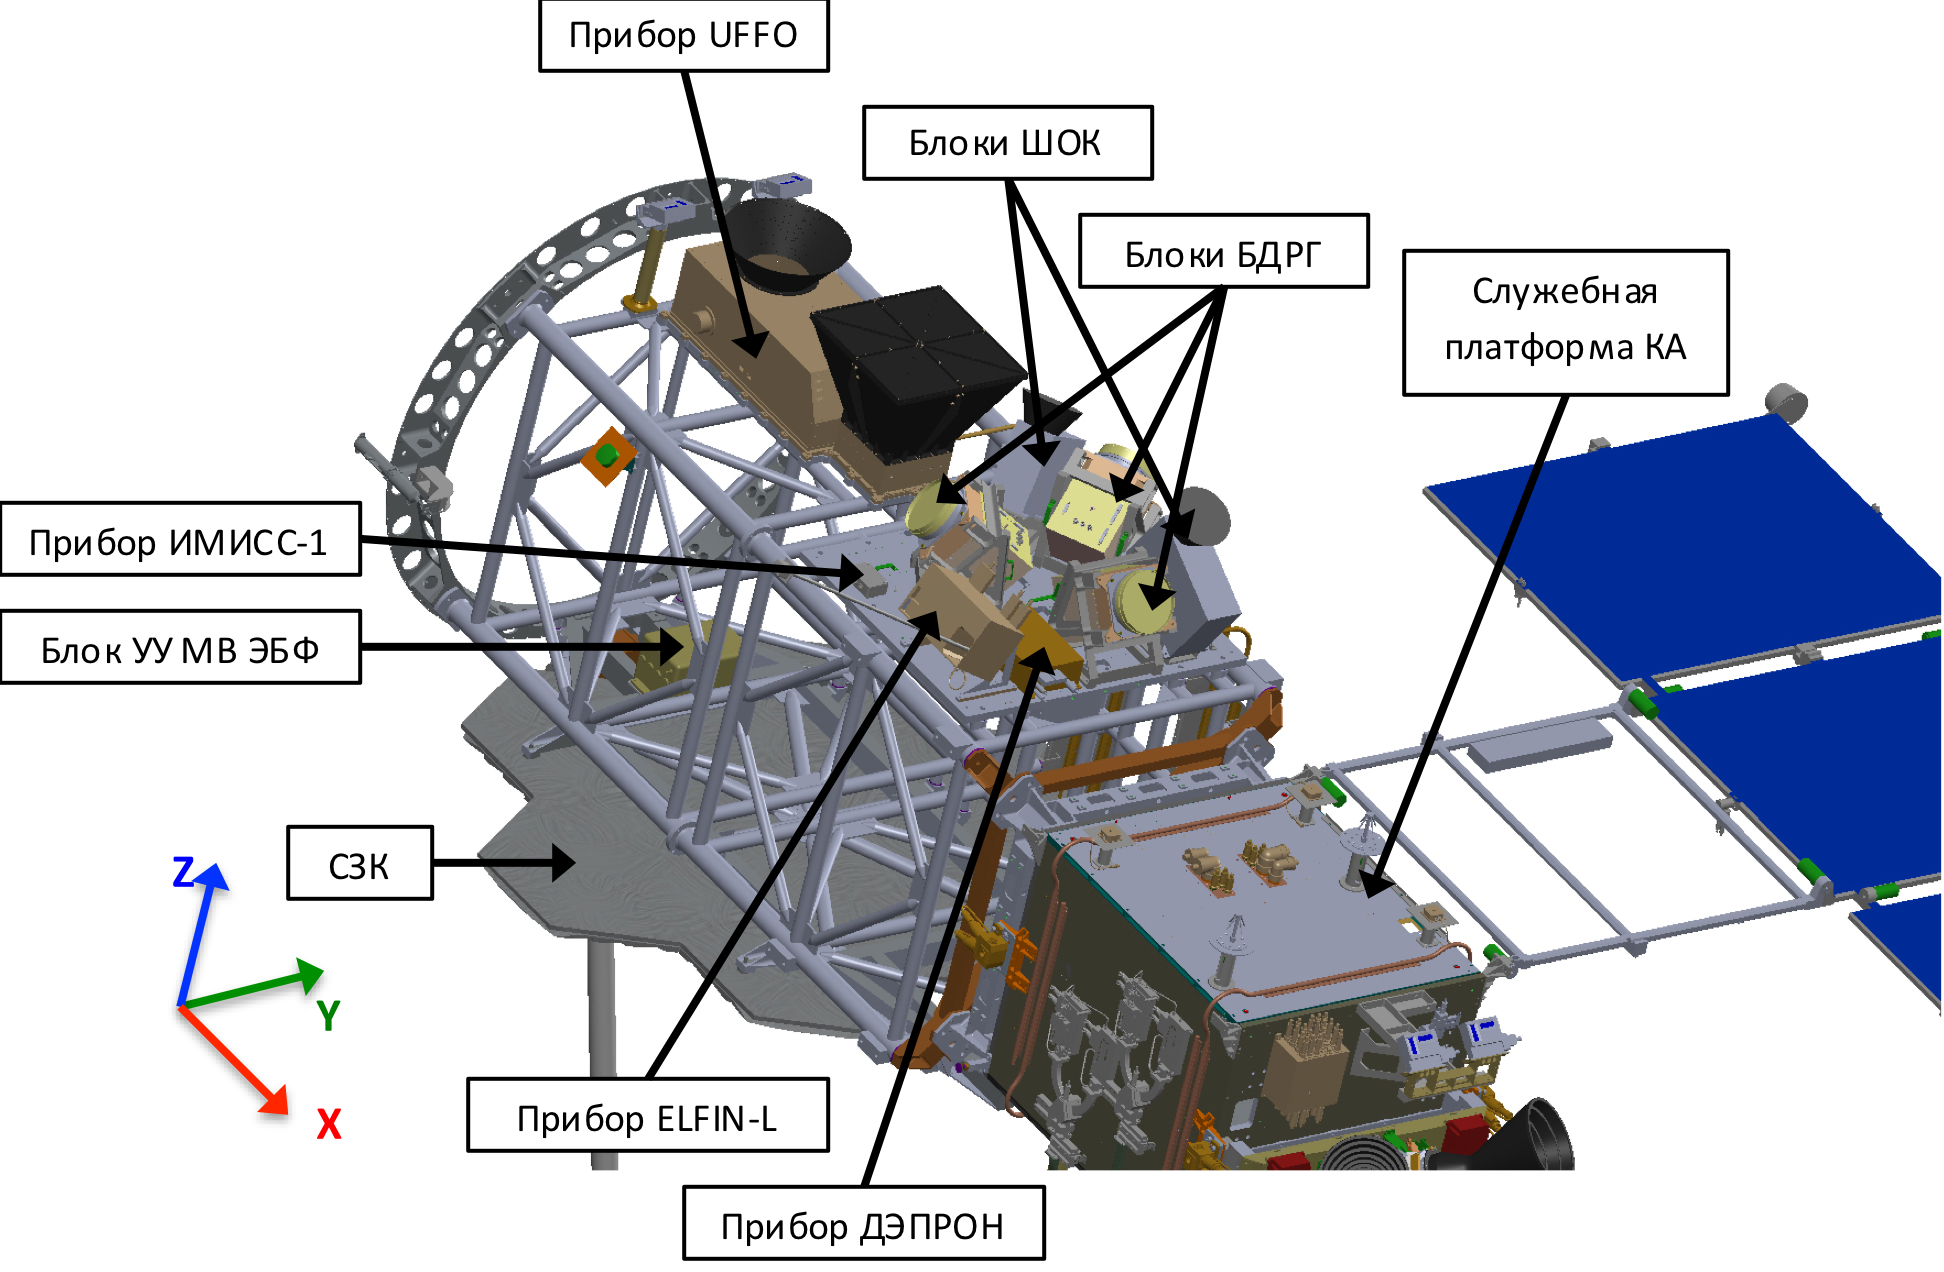
\includegraphics[width=0.9\linewidth]{images/lomo3}
\caption{Внешний вид спутника Ломоносов}
\label{fig:lomo3}
\end{figure}


